\documentclass[tikz,border=2pt]{standalone}
\usepackage{amsmath,amssymb}
\usepackage{tikz}
\usetikzlibrary{arrows.meta}

\begin{document}
% The multiplication principle: 2 choices of shirt times 3 choices of trousers give 2 x 3 = 6
% outfits, one per path through the tree.
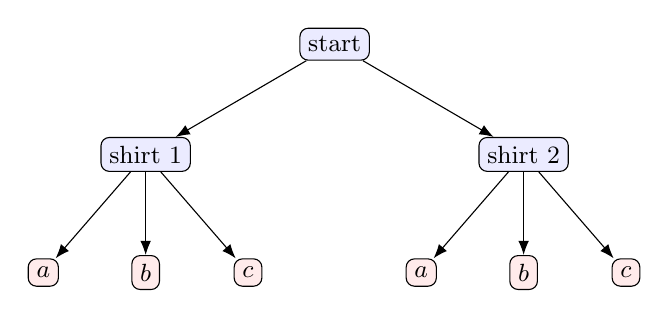
\begin{tikzpicture}[every node/.style={font=\small}, >={Latex[length=1.8mm]}, lvl/.style={draw, rounded corners=3pt, fill=blue!8, inner sep=3pt}]
	\node[lvl] (root) at (0,0) {start};
	\node[lvl] (s1) at (-2.4,-1.4) {shirt $1$};
	\node[lvl] (s2) at (2.4,-1.4) {shirt $2$};
	\draw[->] (root) -- (s1);
	\draw[->] (root) -- (s2);
	\foreach \s/\x in {s1/-2.4, s2/2.4} {
		\node[lvl, fill=red!8] (\s a) at (\x-1.3,-2.9) {$a$};
		\node[lvl, fill=red!8] (\s b) at (\x,-2.9) {$b$};
		\node[lvl, fill=red!8] (\s c) at (\x+1.3,-2.9) {$c$};
		\draw[->] (\s) -- (\s a);
		\draw[->] (\s) -- (\s b);
		\draw[->] (\s) -- (\s c);
	}
	
\end{tikzpicture}
\end{document}
